\documentclass[12pt, twosides]{report}

\usepackage{graphicx}
\graphicspath{ {figures/} }
\usepackage[left=2.5cm,right=2cm,top=2.5cm]{geometry}


\usepackage[utf8]{inputenc}
\usepackage{t1enc}
\usepackage[magyar]{babel}
\linespread{1.5}

\usepackage{footnote}
\usepackage{subfigure}
\usepackage{float}
\usepackage[]{algorithm2e}
\usepackage{amsmath}
\usepackage{mathptmx}
\usepackage{pdfpages}

\usepackage{xcolor}
\usepackage{hyperref}
\hypersetup{
    colorlinks,
    linkcolor=black,
    citecolor=black,
	urlcolor={blue!80!black},
	unicode=true
}
% 
\urlstyle{same}

\usepackage{listings}
\definecolor{dkgreen}{rgb}{0,0.6,0}
\definecolor{gray}{rgb}{0.5,0.5,0.5}
\definecolor{mauve}{rgb}{0.58,0,0.82}
\definecolor{light-gray}{gray}{0.25}

\lstdefinestyle{yaml}{	
	backgroundcolor=\color{white}, % choose the background color;
	basicstyle=\fontsize{8}{8}\ttfamily,% the size of the fonts that are used for the code
	breakatwhitespace=false, % sets if automatic breaks should only happen at whitespace
	breaklines=true, % sets automatic line breaking
	commentstyle=\color{dkgreen},  % comment style
	deletekeywords={...},  % if you want to delete keywords from the given language
	escapeinside={\%}{)},  % if you want to add LaTeX within your code
	extendedchars=true,  % lets you use non-ASCII characters; for 8-bits encodings only, does not work with UTF-8
	frame=none,	 	 % adds a frame around the code
	keepspaces=true, % keeps spaces in text, useful for keeping indentation of code (possibly needs columns=flexible)
	keywordstyle=\color{blue}\bfseries, % keyword style
	otherkeywords={*,...}, % if you want to add more keywords to the set
	numbers=none,  % where to put the line-numbers; possible values are (none, left, right)
	numbersep=5pt, % how far the line-numbers are from the code
	numberstyle=\tiny\color{gray}, % the style that is used for the line-numbers
	rulecolor=\color{black}, % if not set, the frame-color may be changed on line-breaks within not-black text (e.g. comments (green here))
	showspaces=false,% show spaces everywhere adding particular underscores; it overrides 'showstringspaces'
	showstringspaces=false,  % underline spaces within strings only
	showtabs=false,  % show tabs within strings adding particular underscores
	%stepnumber=1,  % the step between two line-numbers. If it's 1, each line will be numbered
	stringstyle=\color{mauve}, % string literal style
	tabsize=2,
	columns=fullflexible  % Using fixed column width (for e.g. nice alignment)
	sensitive = true,
	morekeywords={name, runs-on, on, jobs, build, run, steps, uses}
}
\lstset{style=yaml}

\title{
	{Drónok irányítása}\\
	{\large Sapientia\\
	Erdélyi Magyar Tudományegyetem, Marosvásárhely}
}
\author{
	Vasi, András\\
	\texttt{vasi.andras@student.ms.sapientia.ro}	
}

%%%%%%%%%%%%%%%%%%%%%%%%%%%%%%%%%%%%%%%%%%%%%%%%%%%%%%%%%%%%%%%%%%%%%%%%%

\begin{document}

\pagenumbering{gobble}

\tableofcontents

\listoffigures

\section{Bevezető}
Az utóbbi évtizedek technológiai fejlődése alapvetően megváltoztatta mindennapjainkat, különösen az autonóm járművek és a drónok területén. A drónok, vagy más néven pilóta nélküli légijárművek (UAV-k), egyre elterjedtebbé váltak különféle iparágakban és alkalmazásokban. A mezőgazdaságtól kezdve a katasztrófavédelemig, a filmipartól a haditechnikáig számos területen használják őket hatékonyságuk és sokoldalúságuk miatt.

A drónok irányítása és vezérlése az egyik legizgalmasabb és leginnovatívabb kutatási terület, amely számos tudományágat ötvöz, mint például a robotika, az elektronika, a mesterséges intelligencia és a távközlés. Ahhoz, hogy egy drón képes legyen irányított vagy autonóm módon repülni és különböző feladatokat ellátni, fejlett algoritmusokra és érzékelőkre van szükség. Ezen rendszerek fejlesztése és integrációja komoly mérnöki kihívást jelent, ugyanakkor lehetőséget kínál új technológiák és megoldások kifejlesztésére.

Projekten célja egy saját tervezésű drón létrehozása, amely képes távirányított, majd későbbiekben akár autonóm módon repülni, navigálni és különböző feladatokat elvégezni. A drón építése és fejlesztése során a legújabb technológiákat és módszereket alkalmaztam, mint például a drón 3D fizikai modellezése, 3D kivitelezése (nyomtatása 3D nyomtatóval), irányítási algoritmusok szimulálása MATLAB környezetben. Terveim szerint, ezekkel a technológiákkal egy olyan rendszert hozhatunk létre, amely megbízható és hatékony a valós környezetben történő alkalmazás során. A projekt során különös figyelmet fordítottam a drón irányítási rendszerének kidolgozására és szimulációjára, amely magában foglalja az érzékelők adatainak feldolgozását, a navigációs algoritmusok fejlesztését, valamint a kommunikációs és vezérlő rendszerek integrációját.

A projekt egyik fő kihívása az, hogy olyan irányítási rendszert hozzak létre, amely képes közel valós időben reagálni a környezeti változásokra és az előre nem látható helyzetekre. 


\chapter{Irodalmi áttekintés}
Az utóbbi években a drónok tervezésének területe jelentős fejlődésen ment keresztül, amelyet a kutatások és technológiai innovációk növekvő mennyisége és minősége táplált. Az átfogó szakirodalmi áttekintések sokoldalú alkalmazásokat és technológiai fejlesztéseket tártak fel.

Például a megfigyelési célú drónokkal kapcsolatos kutatások kiemelik a nehezebb-légkörű (Heavier-Than-Air, HTA) és a könnyebb-légkörű (Lighter-Than-Air, LTA) UAV-rendszerek közötti különbségeket. Az ilyen kutatások egyre inkább a kettős rendszerek alkalmazását javasolják, amelyek ötvözik mindkét kategória előnyeit, például a HTA drónok mozgékonyságát és az LTA rendszerek energiahatékonyságát.

További szisztematikus irodalom-áttekintések hangsúlyozzák a dróntechnológia folyamatos fejlődését az elmúlt évtized során. Ezek az áttekintések nem csupán az új technológiák bevezetéséről számolnak be, hanem a drónok alkalmazási körének folyamatos bővüléséről is, különös tekintettel az ipari, mezőgazdasági, logisztikai és környezetvédelmi területekre.

Külön figyelmet érdemelnek a drónok logisztikai alkalmazásairól szóló kutatások, amelyek rávilágítanak ezen eszközök lehetőségeire az árukészlet-ellenőrzés, az utolsó kilométeres kiszállítás és a fenntarthatóság terén. Ezek a tanulmányok alátámasztják, hogy a drónok hatékonyan támogathatják az ellátási lánc optimalizálását, miközben csökkentik a környezeti terhelést, például az üvegházhatású gázok kibocsátását.

E kutatások összességében a dróntervezés dinamikus és folyamatosan fejlődő természetét tükrözik, előkészítve az utat a jövőbeni innovációk és gyakorlati alkalmazások számára. A különböző fejlesztési irányok, mint például az autonóm navigáció, az energiatárolási technológiák javítása és az érzékelőrendszerek integrációja, tovább fokozzák a drónok potenciálját, hogy alapvető szereplőkké váljanak a modern ipari és társadalmi környezetben.
\cite{tadic2021application}, \cite{doornbos2024drone}, \cite{adorni2021literature}

\section{Szabályozási algoritmusok áttekintése: Hagyományos és modern megközelítések}

A szabályozási algoritmusok kulcsszerepet töltenek be számos mérnöki és technológiai alkalmazásban, mivel hatékony eszközt nyújtanak rendszerek és folyamatok irányításához. Az egyik legszélesebb körben alkalmazott szabályozási algoritmus a Proporcionális-Integráló-Deriváló (PID) szabályozó. A PID szabályozók egyszerűségükről és sokoldalúságukról ismertek, legyen szó ipari automatizálásról vagy robotikáról. Ezek az algoritmusok a kívánt érték (setpoint) és az aktuális folyamatváltozó közötti eltérés alapján állítják be a szabályozási jelet, a proporcionális, integráló és deriváló tagok segítségével minimalizálva az eltérést. A PID szabályozók hangolása széles körben kutatott terület, számos módszert dolgoztak ki a teljesítményük optimalizálására1.

Egy másik jelentős szabályozási algoritmus a modell-alapú prediktív szabályozás (Model Predictive Control, MPC), amely népszerűsége a többváltozós rendszerek és a korlátozások kezelésére való képességéből fakad. Az MPC egy dinamikus folyamatmodellt használ a rendszer jövőbeni viselkedésének előrejelzésére, és minden szabályozási lépésben egy optimalizálási problémát old meg az optimális szabályozási akciók meghatározására. Ez az előrelátó megközelítés lehetővé teszi az MPC számára, hogy proaktívan reagáljon jövőbeli eseményekre, így különösen alkalmas komplex ipari folyamatok és fejlett gyártórendszerek szabályozására2. Az MPC rugalmassága és robusztussága miatt széles körben alkalmazzák többek között vegyészmérnöki, autóipari és repülőgépipari rendszerekben.

Az intelligens szabályozási algoritmusok, például a fuzzy logikán, neurális hálózatokon és genetikus algoritmusokon alapuló megoldások szintén jelentős fejlődésen mentek keresztül. Ezek az algoritmusok a biológiai folyamatokat utánozva képesek kezelni a bizonytalanságokat és a nemlinearitásokat a szabályozási rendszerekben. Például a fuzzy logikán alapuló szabályozók nyelvi szabályokkal modellezik a komplex rendszereket, ami különösen hasznos azokban az alkalmazásokban, ahol a pontos matematikai modellek nehezen elérhetők3. A neurális hálózatok ezzel szemben képesek adatokból tanulni és alkalmazkodni a változó körülményekhez, így erőteljes eszközt kínálnak az adaptív szabályozás számára. A genetikus algoritmusok a természetes szelekció folyamatát szimulálva optimalizálják a szabályozási paramétereket3.

A hagyományos és intelligens szabályozási algoritmusok mellett egyre nagyobb figyelmet kapnak a hibrid szabályozási rendszerek, amelyek több szabályozási stratégia kombinációját használják azok előnyeinek kihasználására. Például a PID szabályozók és a fuzzy logika kombinálása javíthatja a szabályozási rendszer teljesítményét, egyszerre biztosítva precíz szabályozást és robusztusságot a bizonytalanságokkal szemben. Hasonlóképpen, az MPC és a neurális hálózatok integrációja növelheti a szabályozási rendszer előrejelzési pontosságát és alkalmazkodóképességét2. Ezek a hibrid megközelítések különösen hasznosak komplex és dinamikus környezetekben, ahol egyetlen szabályozási stratégia nem elegendő.

A szabályozási algoritmusok folyamatos fejlődését a számítástechnika teljesítményének növekedése és a modern rendszerek növekvő komplexitása hajtja. Ahogy az iparágak a smart manufacturing és az Ipar 4.0 irányába haladnak, egyre nagyobb az igény olyan fejlett szabályozási algoritmusokra, amelyek képesek nagy léptékű, összekapcsolt rendszereket kezelni. A kutatások célja hatékonyabb és skálázhatóbb algoritmusok fejlesztése, valamint új alkalmazási területek feltárása az autonóm járművek, a megújuló energiaforrások és a Dolgok Internete (IoT) terén. A jövő szabályozási algoritmusai várhatóan képesek lesznek alkalmazkodni a változó körülményekhez, tanulni az adatokból, és valós időben biztosítani az optimális teljesítményt.

\cite{lee2023review}, \cite{schwenzer2021review}, \cite{borase2021review}

\chapter{A projekt leírása}
Jelenleg egy saját fejlesztésű drón építésén dolgozom, ezen egyetemi tantárgy keretében valósul meg. A drón fizikailag már megépült nagyjából, a konstrukcióhoz 3D nyomtatott technológia került alkalmazásra. A fejlesztés előzménye szakirodalmi kutatás volt, mely során különböző dróntechnológiák és szabályozási módszerek kerültek áttekintésre. A drón szimulációja MATLAB Simulink környezetben zajlik, amely lehetővé teszi a különböző rendszerek és vezérlési algoritmusok modellezését.

Bár a drón még nem készült el teljesen, a projekt folyamatban van, és az építés előrehaladott állapotban van. A drón jelenlegi formája még további finomításra szorul, és számos lehetőség rejlik a fejlesztésében. Az aktuális verzióval kapcsolatosan több szempontból is van lehetőség a teljesítmény javítására, különösen a vezérlőrendszerek optimalizálása, az akkumulátor élettartamának növelése és az irányíthatóság fokozása terén.

A drón befejezése várhatóan a közeljövőben megtörténik, és az egyetemi projekt célja, hogy lehetőséget adjon a valós idejű alkalmazások tesztelésére, valamint további fejlesztési irányok feltárására is. A projekt nemcsak technológiai kihívásokat tartogat, hanem számos lehetőséget is biztosít a drónokkal kapcsolatos kutatások és alkalmazások mélyebb megértésére.

\chapter{Drón tervezése és felépítése}
\section{Tartószerkezet és 3D nyomtatott váz}

A drónok tervezése és építése során az egyik legfontosabb szempont a stabil és megbízható tartószerkezet kialakítása. Az alkalmazott anyagok és technológiák döntően befolyásolják a drón repülési jellemzőit, terhelhetőségét és élettartamát. A projektünk során a 3D nyomtatási technológiát választottuk a váz és a tartószerkezet létrehozásához, mivel ez a módszer számos előnyt kínál a hagyományos gyártási technikákkal szemben.

Az alkalmazott 3D nyomtatási technológia lehetővé teszi a komplex geometriák és precíz részletek létrehozását, amelyek különösen fontosak a drón szerkezetének optimalizálása és a súlycsökkentés szempontjából. A 3D nyomtatott váz könnyű, mégis rendkívül erős, ami hozzájárul a drón stabil repülési tulajdonságaihoz és hosszú élettartamához.

A drón vázát 70\%-os kitöltéssel nyomtattuk PET-G anyagból, amely erős és ellenálló, miközben megőrzi a szükséges rugalmasságot és könnyűséget. Az egyes aklatrészek rögzítése egymáshoz 16 darab M5-ös 20 miliméteres hexagon fejű csavarral és M5-ös anyával történt. 

\begin{figure}[H]
	\centering
	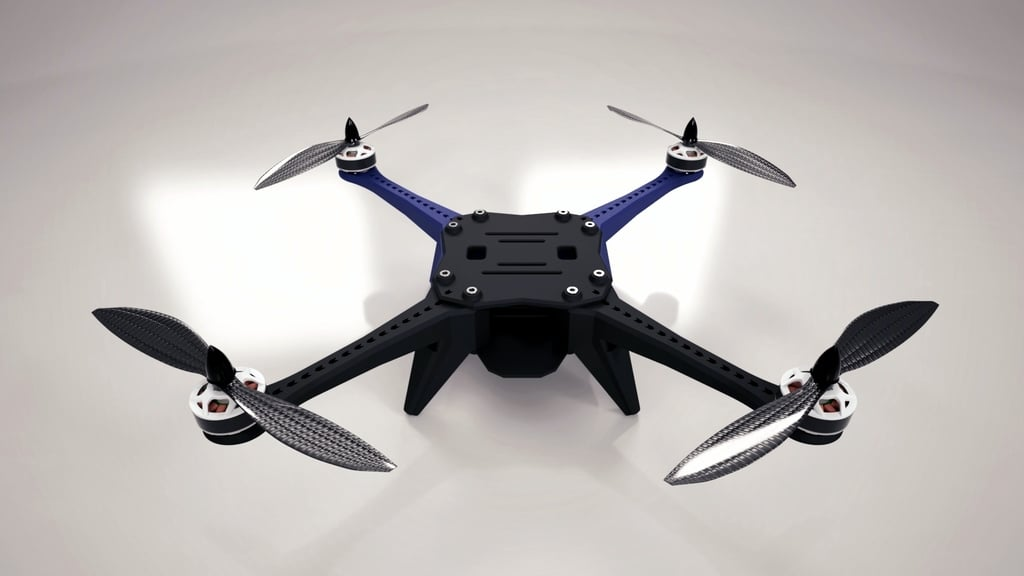
\includegraphics[scale=0.3]{figures/drone_model.JPG}
	\caption{A drón 3D -s modellje}
	\label{A drón 3D -s modellje}
\end{figure}

\section{Elektronikai aklatrészek}

Az alábbiakban a drón motorjairól, elektronikus fordulatszám-szabályozóiról (ESC), az akkumulátorról, valamint a központi vezérlőegységről esik szó.

\subsection{BLDC motorok}
A drón meghajtását négy darab kefe nélküli egyenáramú (Brushless DC, BLDC) motor biztosítja. Ezek a motorok a magas hatékonyságuk és tartósságuk miatt ideálisak drónokhoz. A kefe nélküli kialakítás előnye, hogy minimalizálja a mechanikai kopást, így hosszabb élettartamot és kevesebb karbantartást igényel.

A motorok forgómágneses rendszere és a szállítólégcsavarok (propellerek) közvetlenül a drón stabilitásáért felelősek. A négy motor együttműködése lehetővé teszi a drón emelkedését, süllyedését, valamint forgását és előre-hátra irányuló mozgását.


\begin{figure}[H]
	\centering
	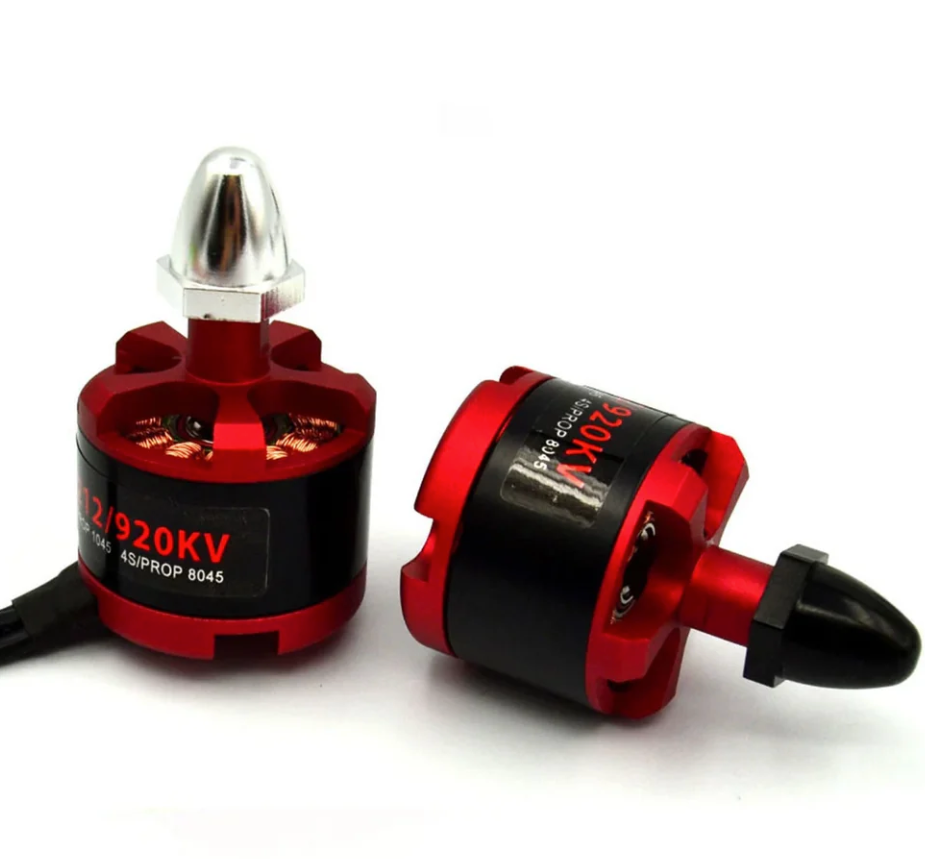
\includegraphics[scale=0.3]{bldc_motor.png}
	\caption{Drónhoz felhasznált BLDC motrok}
	\label{Drónhoz felhasznált BLDC motrok}
\end{figure}

\subsection{ESC-k}
A motorok működését négy elektronikus fordulatszám-szabályozó (Electronic Speed Controller, ESC) vezérli. Az ESC-k feladata, hogy az akkumulátorból érkező elektromos energiát a motorok számára megfelelő frekvenciájú és amplitódójú jelré alakítsák. Ezáltal az ESC-k precíz szabályozást biztosítanak a motorok forgási sebességéhez, ami kulcsfontosságú a drón stabilitása és irányíthatósága szempontjából.

Az általam használt ESC-k beépített védelmi mechanizmusokkal rendelkeznek, amelyek megakadályozzák a túlmelegedést és a túláram miatti meghibásokat. Továbbá, ezek a szabályozók kompatibilisek a BLDC motorokkal, ami garantálja a rendszer zavartalan működését.

\begin{figure}[H]
	\centering
	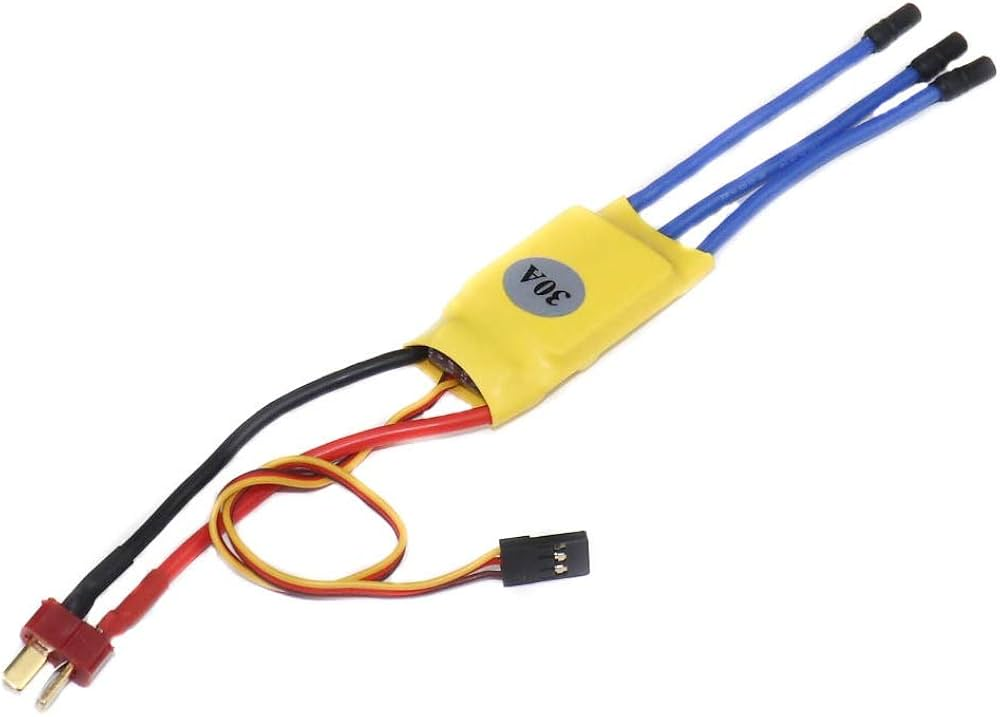
\includegraphics[scale=0.3]{esc.jpg}
	\caption{Drónhoz felhasznált ESC-k}
	\label{Drónhoz felhasznált ESC-k}
\end{figure}

\subsection{Akkumulátor}
A drón energiaellátását egy nagy kapacitású lítium-polimer (LiPo) akkumulátor biztosíthatja. Az akkumulátor kiválasztásakor figyelembe kell venni a drón súlyát, a motorok áramfogyasztását és a kívánt repülési időt. A LiPo akkumulátorok előnye, hogy magas energiasűrűséggel rendelkeznek, ami lehetővé teszi a hosszabb repülési időt anélkül, hogy jelentős súlyt adnának a drónhoz.

\begin{figure}[H]
	\centering
	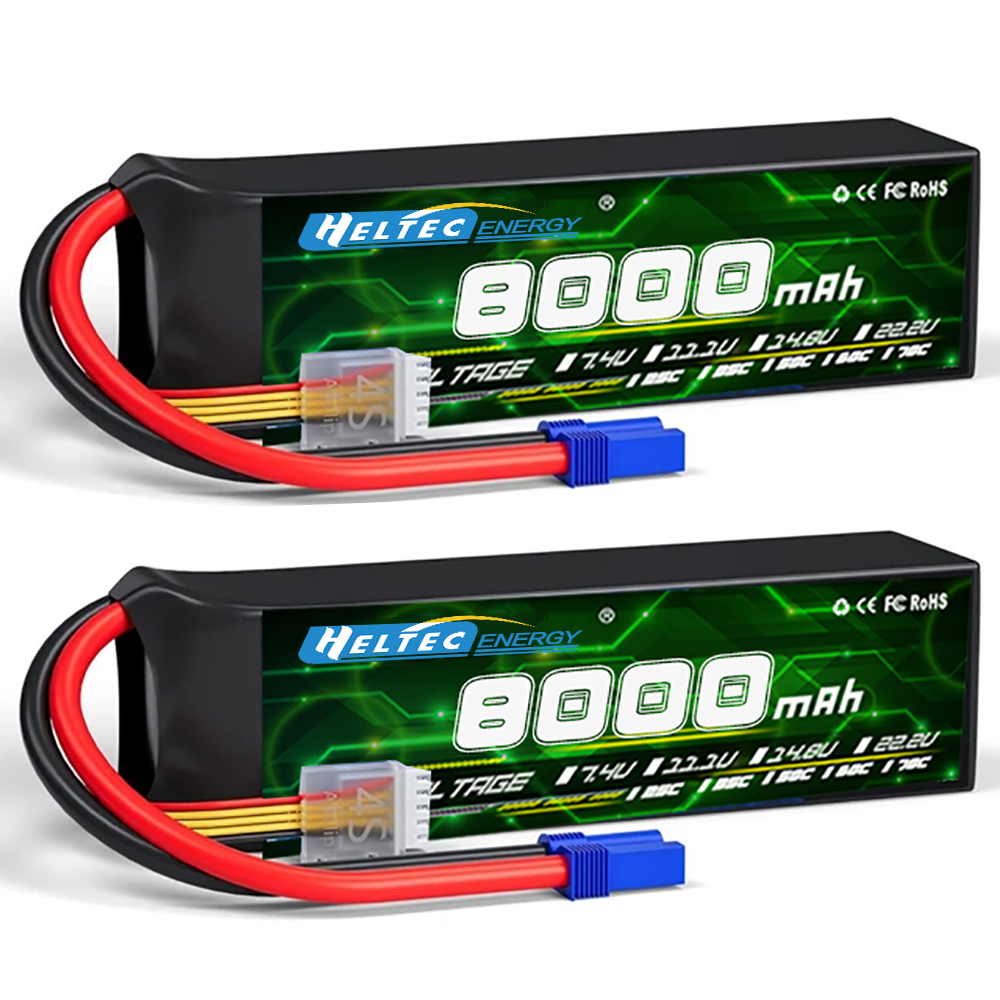
\includegraphics[scale=0.25]{battery.jpg}
	\caption{Drónhoz felhasználható akkumulátorok}
	\label{Drónhoz felhasznált ESC-kDrónhoz felhasználható akkumulátorok}
\end{figure}

\subsection{Központi vezérlőegység}
A drón "agya" a központi vezérlőegység, amely a rendszer minden elemét összehangolja. 

Ez a vezérlőegység tartalmazza a drón stabilitását biztosító algoritmusokat, így mint a PID szabályozást, amely minimalizálja a lengéseket és stabilizálja a drónt repülés közben. Továbbá, a vezérlőegység kapcsolódik a távirányítóhoz és a GPS modulhoz, ami lehetővé teszi az automatikus és manuális repülési módok közötti váltást.

\subsubsection{IMU (Inerciális mérőegység)}
Az IMU (Inertial Measurement Unit) egy kulcsfontosságú szenzor, amely a drón mozgásának és orientációjának pontos mérését végzi. Az IMU tipikusan gyorsulásmérőket (accelerometer), giroszkópokat (gyroscope) és néha magnetométereket is tartalmaz, amelyek segítségével az alábbi adatokat méri:

Lineáris gyorsulás: A drón mozgási sebességének változása az x, y és z tengelyek mentén.

Szögsebesség: A drón forgási sebessége a giroszkóp adatai alapján, amely a roll, pitch és yaw tengelyeken történő forgást méri.

Mágneses mező iránya: A magnetométer segítségével meghatározható a drón relatív iránya a Föld mágneses teréhez képest.

Az IMU által mért adatok valós időben kerülnek feldolgozásra a központi vezérlőegységben. Ezek az adatok nélkülözhetetlenek a drón stabilitásának fenntartásához és pontos irányításához. A vezérlőegység a kapott értékeket folyamatosan elemzi, és szükség esetén korrigálja a motorok sebességét a megfelelő stabilitás és iránytartás érdekében.

A gyorsulásmérő adatai segítenek a drón helyzetének meghatározásában, míg a giroszkóp adatai a forgás stabilizálásában játszanak szerepet. A magnetométer, ha rendelkezésre áll, további pontosságot biztosít az iránymeghatározásban, különösen akkor, ha a drón GPS-alapú navigációt végez.

Az IMU által szolgáltatott pontos és gyors adatok lehetővé teszik, hogy a drón dinamikusan alkalmazkodjon a környezeti változásokhoz, például szélmozgáshoz vagy hirtelen irányváltásokhoz, biztosítva ezzel a megbízható és zökkenőmentes repülést.

\subsubsection{Kalman-szűrő}
A Kalman-szűrő egy matematikai algoritmus, amelyet a drón vezérlőegysége használ az IMU és más szenzorok által szolgáltatott adatok pontosítására és zajcsökkentésére. Ez az algoritmus különösen fontos a drón repülési stabilitásának és irányításának biztosításához, mivel a szenzorok adatai gyakran zajosak és pontatlanok lehetnek.

A Kalman-szűrő az alábbi lépéseket hajtja végre:

Előrejelzés: A rendszer aktuális állapotából (például pozíció, sebesség, orientáció) előrejelzi a következő állapotot egy dinamikai modell alapján.

Mérés: Az IMU és más szenzorok új adatokat szolgáltatnak az aktuális állapotról.

Frissítés: Az előrejelzett állapotot összehasonlítja a mért adatokkal, és korrigálja az előrejelzést, figyelembe véve a szenzorok pontosságát és a mérési zajt.

A Kalman-szűrő alkalmazásával a drón vezérlőegysége képes pontosabb állapotbecslésre, amely alapját képezi a stabil repülésnek és a precíz irányításnak. Például, ha az IMU giroszkópja és gyorsulásmérője kissé eltérő adatokat ad, a Kalman-szűrő a két forrás kombinációjával egy pontosabb képet nyújt a drón valódi mozgásáról.

Ez az algoritmus kulcsfontosságú a dinamikus környezetekben, ahol a drónnak gyorsan és pontosan kell reagálnia a külső hatásokra, például szélre vagy akadályokra. A Kalman-szűrő alkalmazása jelentősen javítja a rendszer megbízhatóságát és teljesítményét, különösen az autonóm repülési funkciók esetében.

\chapter{Irányítási rendszer}
\input{chapters/iranyitasi_rendszer}

\chapter{Szimuláció}
\section{A drón kontroller modellje MATLAB Simulinkben}
A drón vezérlőrendszerének modellezését és szimulációját MATLAB Simulink környezetben végeztem el, az UAV Toolbox segítségével. Ez az eszközkészlet kifejezetten hasznos a drónok és más légi járművek fejlesztése során, mivel előre elkészített modulokat és sablonokat kínál a vezérlési, navigációs és repülésdinamikai modellezéshez.

\begin{figure}[H]
	\centering
	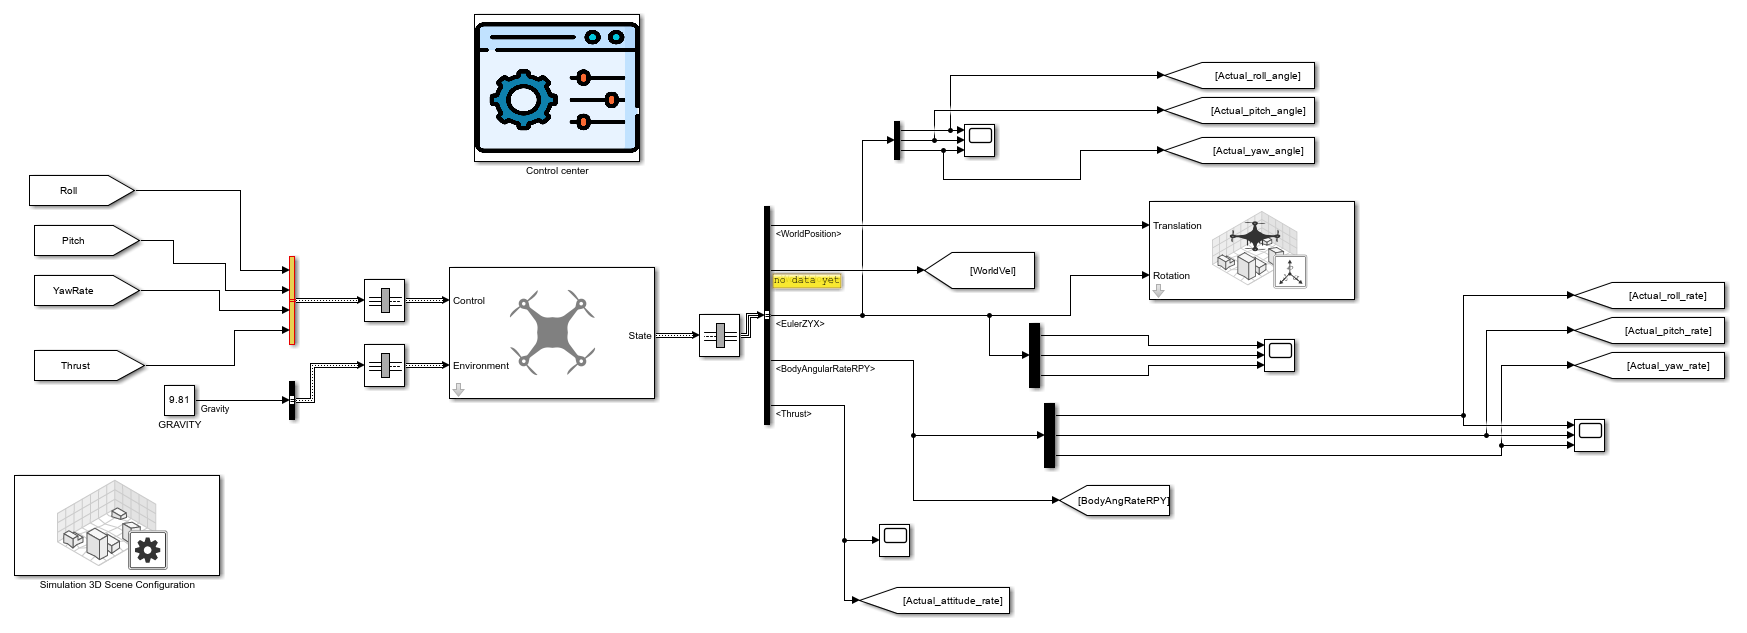
\includegraphics[scale=0.3]{control-arch.png}
	\caption{Drón kontroller architechtúrája}
	\label{Drón kontroller architechtúrája SIMULINK környezetben}
\end{figure}

\begin{figure}[H]
	\centering
	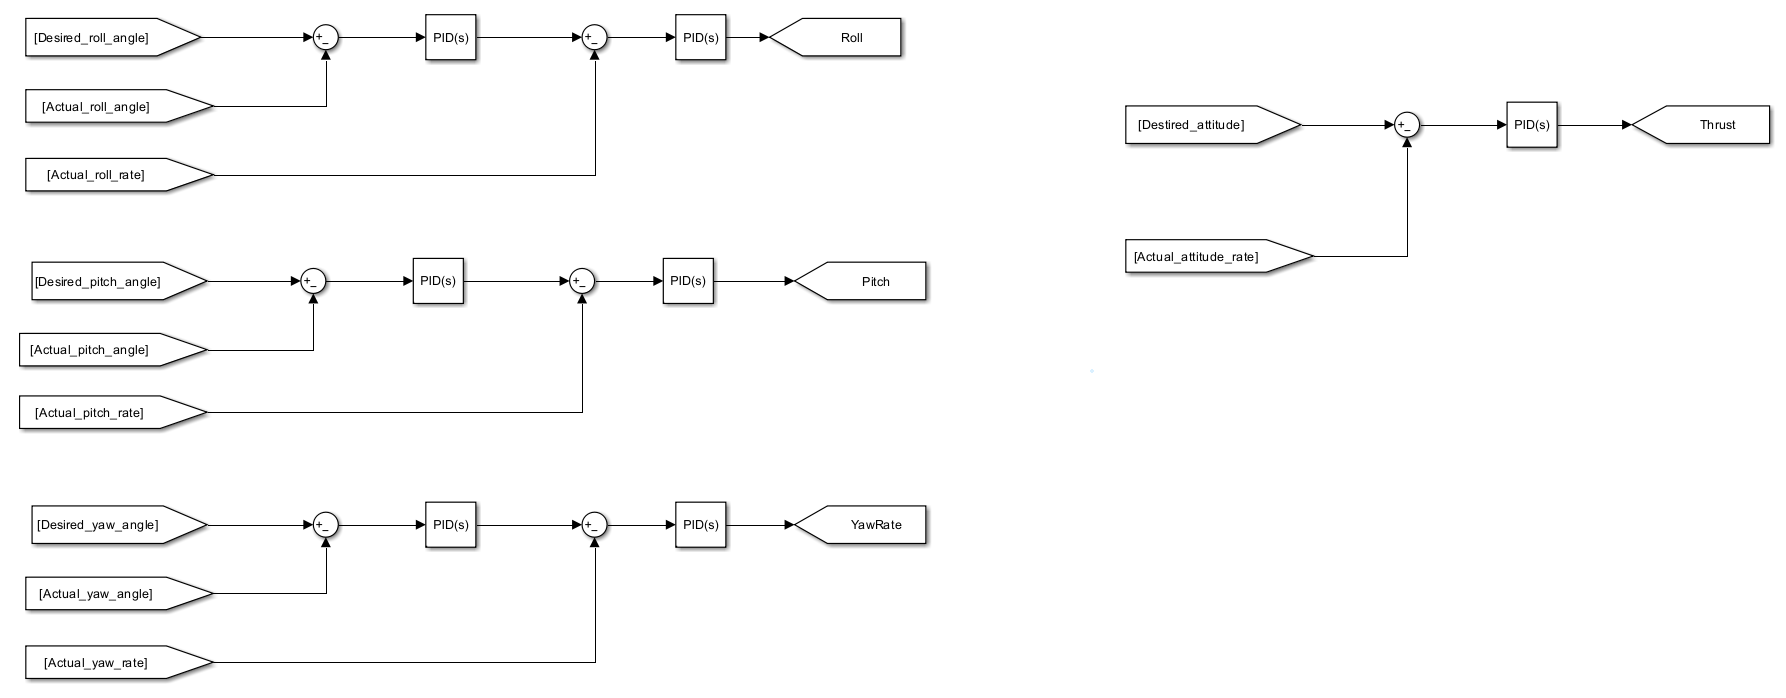
\includegraphics[scale=0.3]{cascade-pid-control.png}
	\caption{Drón visszacsatolt rendszerének cascade szabályzása}
	\label{Drón visszacsatolt rendszerének cascade szabályzása}
\end{figure}


\chapter{Megvalósítás és tesztelés}
\begin{figure}[H]
	\centering
	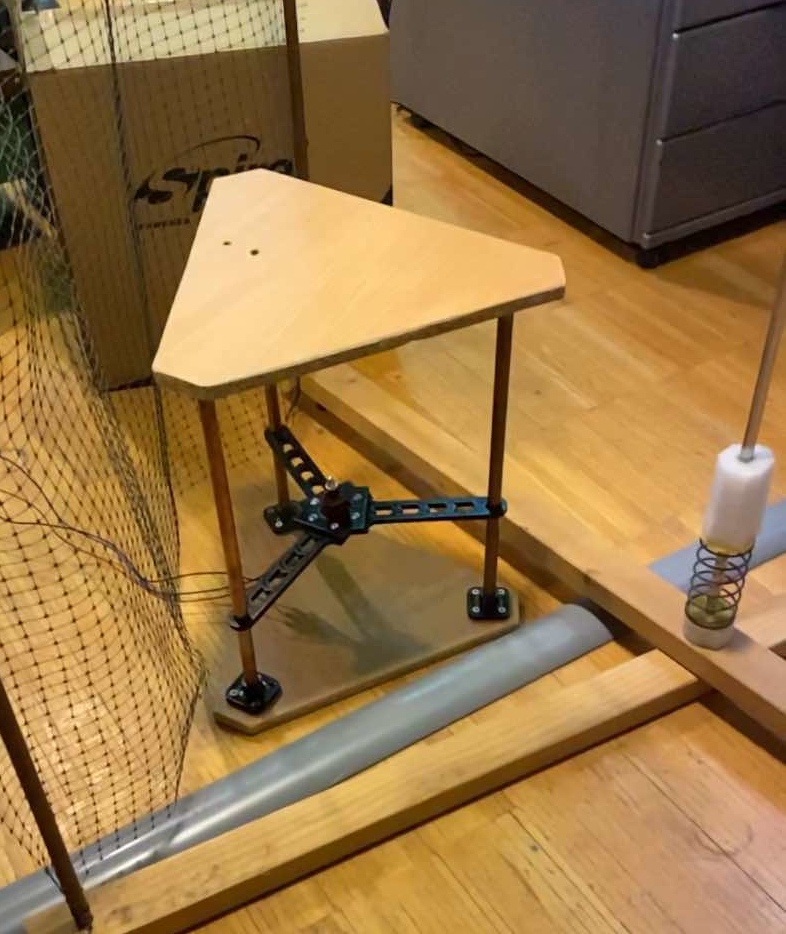
\includegraphics[scale=1]{simpad.jpg}
	\caption{Drón szabályzásának vizsválatára használt berendezés}
	\label{Drón szabályzásának vizsválatára használt berendezés}
\end{figure}


\chapter{Eredmények és értékelés}
Az egyetemi tárgy keretében olyan projektet választottam, amely a drónok irányítását és fejlesztését állítja a középpontba. A projekt célja egy saját tervezésű és készítésű drón megépítése, szimulációs környezetben történő tesztelése, valamint a repülési képességek és az autonóm irányítás alapjainak kidolgozása. Ez a fejezet a projekt jelenlegi állapotát, a megvalósított részleteket és a felmerült kihívásokat ismerteti.

A drón majdnem teljes egészében saját tervezésű, a fő szerkezeti elemek 3D nyomtatással készültek. A kivitelezés során nagy hangsúly került a stabilitásra és a szerkezeti integritásra, mivel ezek alapvetõen befolyásolják a drón repülési tulajdonságait. Az elektronikai komponensek közül az irányítási rendszert és a szenzorokat a projekt összetettségének megfelelően választottam ki. A drón jelenleg még nem képes felszállni, de a szerkezeti és műszaki elemek nagy része már elkészült, és az összeszerelés utolsó fázisában van.

A projekt szerves részét képezi a szimulációs környezet kialakítása, amelyben a drón repülési képességeit és irányítási algoritmusait lehet tesztelni. A MATLAB Simulink használatával igyekeztem modellezni a drón fizikai rendszerét és a környezeti hatásokat. A szimuláció közben azonban számos kihívással szembesültem:

-  rendszer pontossága: A drón dinamikájának modellezése bonyolultabbnak bizonyult, mint azt előzetesen feltételeztem, ami némi eltérést eredményezett a valós viselkedéshez képest.

- Környezeti modellezés: A külső hatások, mint például a szél, turbulencia és gravitáció szimulációja külső források és referenciaanyagok bevonását igényelte.

Ezek a nehezíségek ellenére sikerült létrehozni egy alapvetően működő rendszert, amely alkalmas a további fejlesztések alapjainak lefektetésére.


\chapter{Következtetések és jövőbeli munka}
Bár a drón jelenleg még nem képes a felszállásra, a projekt jelentős előrelépést jelentett a tervezés, szimuláció és kivitelezés területén. A következő lépések közé tartozik:

A szimulációs környezet pontosítása a valós repülési viselkedés jobb megközelítése érdekében.

A drón összeszerelésének befejezése és a mérési eredmények alapján történő optimalizáció.

Az autonóm irányítási algoritmus fejlesztése és implementálása.

A mesterséges intelligencia alkalmazása a rendszerben, amely lehetővé teszi a drón intelligensebb, adaptív irányítását és képes lehet önálló döntéshozatalra is. Ez nemcsak technológiai előrelépést jelentene, hanem trendi megoldásként a projekt piaci értékét is növelné.

A projekt hátralevő részei izgalmas lehetőségeket tartogatnak a további tanulmányok és kísérletek számára, amelyek hozzájárulhatnak a dróntechnológia átfogó megértéséhez.

\chapter{Mellékletek}
\input{chapters/mellekletek}

\addcontentsline{toc}{chapter}{Irodalomjegyzék}
\bibliographystyle{ieeetr}
\bibliography{References}

% \appendix
% \chapter{Függelék}
% \input{chapters/appendix}


\end{document}